\documentclass[a4paper]{article}

\usepackage[utf8]{inputenc}

\usepackage{url}
\usepackage[]{hyperref}

\usepackage{caption}

\usepackage{listings}

\usepackage{color}

% *** GRAPHICS RELATED PACKAGES ***
%\usepackage[pdftex]{graphicx}
\usepackage{graphicx}
%\usepackage[dvips]{graphicx}
% to place figures on a fixed position
\usepackage{float}

\usepackage[margin=1in]{geometry}

\title{OpenFlow \& Mininet – Docker}
\author{}
\date{}


\begin{document}

\maketitle

\tableofcontents

\section{Linux containers}
The Linux Containers (LXC) provide operating system level virtualized environment in which isolated Linux systems
(containers) can be run on the Linux host machine. The operating system level environment virtualization can be viewed
as a lightweight Virtual Machines (VMs). What makes this better compared to VMs? It requires less disk space compared
to a fully virtualized guest OS, provides rapid creation and fast operation. In contrast to emulating the full hardware
environment Containers use a shared, common OS kernel resulting in more efficient runtime performance compared to
full-fledged OS virtualization.

In another aspect it is called ``chroot on streoids". The \emph{chroot} utility runs the specified command or
interactive shell using the root directory specified as command argument. The process run by chroot is quasi ``locked"
inside the specified directory, it can not reach any of the files outside that. This can be used for creating a system
within the system.

\begin{figure}[H]
    \centering
    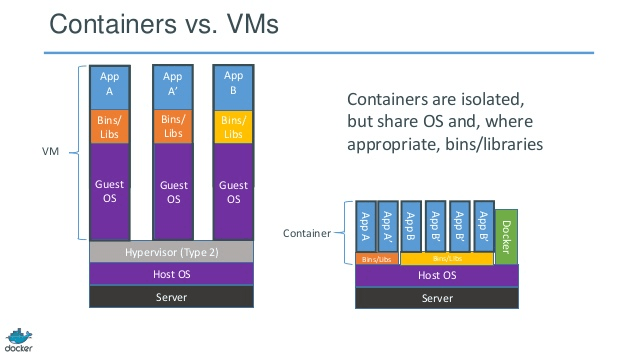
\includegraphics[width=0.9\textwidth]{figures/container_vs_vm.png}
    \caption{Containers vs. VMs}
    \label{fig:containers}
\end{figure}

The Linux kernel's control groups (\emph{cgroups}) function provide facilities for partitioning and prioritizing
resources without having to
start virtual machines. Furthermore with the help of \emph{namespaces} the visibility of file systems, user IDs,
network connections can be
isolated for individual applications. As a result a unique runtime environment can be created for our application that
runs isolated from
the other containers and from the host machine.
The container application's dependencies (software suites, libraries, configuration files) can be embedded into the
container resulting in
highly portable, restartable, manageable unit.
For example one can create a container for a web server, another one for its database, yet another for their message
queue or alternatively these
can be combined into a single container hence allowing the creation of modular application architecture.
If a user packs his self-developed software into a container it can be ensured that the software will be able to
execute on another host machine regardless from the type of the host (developer machine, user machine, application
server etc.) resulting in great flexibility in terms of portability.
If an executable can be executed on a Linux box that can packed into a Linux Container also. Containers provide a new
and easier way of working in application coding, building, installation and execution and can be installed easily on
machines running in a cloud provider's environment.

\section{Docker}

Docker offers an open-source platform for managing containers that can be used for development and execution of
distributed applications
while offering portability.
It provides a common toolset for programmers and development teams and for operations personnel (DevOps) that can
exploit the benefits
of distributed network applications.
The Docker runtime runs as a daemon in the background managing the containers, the images and the creation of those.

The goal of Docker is to simplify the usage of LXC and beside that it allows the containers to be used on different
types of Linux
distributions -- i.e. it abstracts the LXC system specific parts. In the beginning Docker used the LXC format but
currently it uses its own
container format. One important difference between those two formats is that in LXC there is an \emph{init} process as
a consequence multiple
process can be run in it. In contrast Docker doesn't have one so only one process can be run. (For detailed list of
differences please see \url{https://www.flockport.com/lxc-vs-docker/})

Docker's architecture follows the client-server based model as illustrated on Figure~\ref{fig:arch}. The commands
requested by the Docker client are executed by the Docker daemon (engine, server).
The user has no direct interaction with the Docker daemon only through the Docker client this is the ``docker" utility
that provides the
user interface. The client and the daemon can run on the same machine or the client can connect to a remote daemon
process alternatively. The communication can be carried out either over sockets or over RESTful API.

\begin{figure}[H]
    \centering
    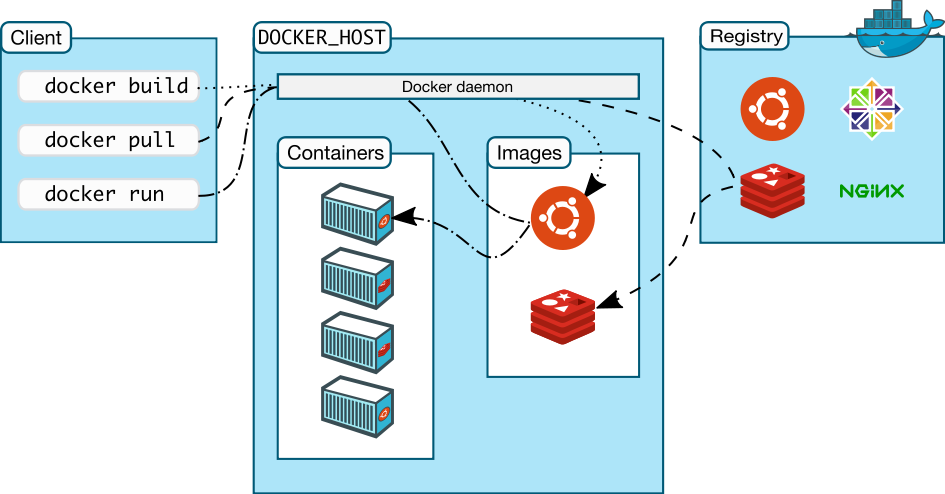
\includegraphics[width=0.9\textwidth]{figures/docker_arch.png}
    \caption{Docker components and architecture}
    \label{fig:arch}
\end{figure}

Docker requires an image file from a given operating system. The image is a write-protected template that is used for
starting the containers.
When running the container this is augmented with an upper layer of writeable filesystem that is used for running the
application. The image file
is basically a pre-installed system that is composed from \emph{aufs} or \emph{btrfs} layers (Union File System) and it
is version controlled as it can be seen on Figure~\ref{fig:layers}.
At startup there is a base image -- e.g. Ubuntu or Debian -- and the all the overlaying file-systems are joined
together to form a final file-system. Additional layers can be placed on any image -- not just the base image -- to
modify that for certain needs. The image files can be created by the user or downloaded from Docker Hub web-page
created by other users. Docker Hub is a public repository but a privately hosted repository can also be used. The
custom made images can be uploaded and shared with the community.

\begin{figure}[H]
    \centering
    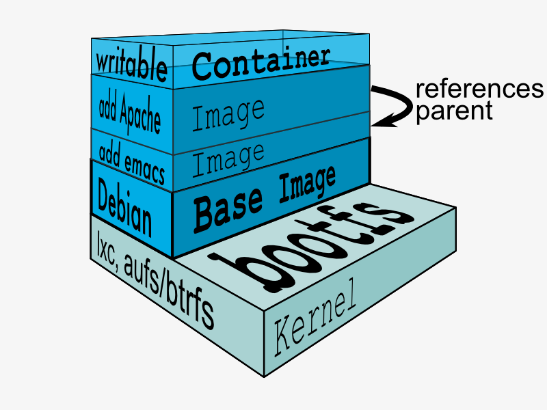
\includegraphics[width=0.9\textwidth]{figures/docker_layers.png}
    \caption{Docker layers}
    \label{fig:layers}
\end{figure}

A container is actually a running entity of a given image. Multiple containers can also be run from the same image file
simultaneously.

Creation and extension of Docker image files can be done in two ways: either by entering into the container manually
and installing and configuring the desired software then by saving the resulting image file or by using a
\emph{Dockerfile} that has a script-like syntax where the
installable components can be declared easily.

\section{Further Reading}

\begin{itemize}
    \item Docker áttekintés: \url{https://docs.docker.com/engine/docker-overview/}
    \item Docker bevezetés: \url{https://docs.docker.com/get-started/} Part 1. and 2.!
\end{itemize}

\appendix

\section{Entry quiz sample questions}

\begin{enumerate}
    \item What is the difference between the VMs and the Linux Containers?
    \item Which Linux kernel functions allow the implementation of containers?
    \item What is the relation between Docker images and containers?
    \item How are Docker images used, who can create them, how can one obtain them?
    \item How are Docker images extended/updated?
    \item What are the purposes of interactive and dameon modes?
    \item What is the difference between docker run and docker start commands?
    \item How are the container network interface mapped to the host machine?
\end{enumerate}

\section{Lab exercises}

\subsection{Lab environment \& introduction}
\subsubsection{List of important commands}

\subsection{Task 1.}
\subsubsection{Application containers}
\subsubsection{Interconnecting two containers}
\subsubsection{Web content and database upload}
\subsection{Task 2.}
\subsection{Task 3.}

\end{document}